% ============================================================================
% Paper 4 -- integrated from papers/IEEE_Conference_MADTECC___Representation_of_Machine_Learning_Models_to_Enhance_
% Simulation_Capabilities_Within_Digital_Twins_in_Personalized_Healthcare/conference_101719.tex (front matter
% transcribed from the IEEEtran author blocks, abstract and IEEEkeywords; inline \thebibliography converted to
% BibTeX entries; body converted mechanically, see the integration report).
% ============================================================================
\papersection{Representation of Machine Learning Models to Enhance Simulation Capabilities Within Digital Twins in Personalized Healthcare}{sec:paper4}

\noindent This section contains the article~\cite{marfoglia_2024_mimo}.

\begin{paperheader}
\textbf{Authors:} Alberto Marfoglia, Filippo Nardini, Sabato Mellone, Antonella Carbonaro.\par
2024 IEEE International Conference on Pervasive Computing and Communications Workshops and Other Affiliated Events (PerCom Workshops), 2024, pp. 100--105. DOI: \url{https://doi.org/10.1109/PerComWorkshops59983.2024.10502444}.
\end{paperheader}

\begin{paperabstract}

Healthcare has always been a strategic area where innovative technologies can be applied to increase the effectiveness of services and the quality of patient care. Recent progress has been made in the adoption of machine-learning models within digital twins and knowledge graphs. Nevertheless, their deployment needs to address the complex nature of the framework itself, which entails numerous technical, organizational, legal, and ethical challenges. In this paper, we propose an evolution of the CONNECTED conceptual framework, a multi-layered system in which heterogeneous data sources are integrated, standardized, and used to realize digital twins supported by knowledge graphs accessible through dedicated APIs. The extension involves the integration of machine learning models into digital twins, thereby enabling simulation capabilities. The inclusion of a formal and machine-readable self-description with these models serves as a foundation for semantic reasoning. This pivotal feature empowers our architecture with the capability for automatic indexing, aggregation, and querying of the models.
\end{paperabstract}

\paragraph{Keywords:} Machine Learning Models, Digital Twins, Personal Knowledge Graphs, Healthcare

\subsection{Introduction}\label{sec:paper4_introduction}

Personalized healthcare is an evolving field of study aimed at delivering targeted treatments and preventive care tailored to each patient's unique medical history, genetic makeup, and specific values \cite{johnson_precision_2021}. Personalized healthcare services have the potential to enhance the quality of life for people worldwide by providing individualized data-driven insights, thereby aiding medical professionals in making more informed decisions. This approach can not only reduce healthcare costs but also drive breakthroughs in all healthcare systems. Artificial Intelligence plays a pivotal role in the realization of personal healthcare services; it is not surprising that its integration in the healthcare sector continues to evolve \cite{sun_review_2022}. To advance the field of personalized healthcare systems, digital twin (DT) solutions can be employed. The DT can excel at identifying subtle, disease-specific patterns from a wide array of sources, optimizing the performance of patient-specific treatment plans, recommending lifestyle advice, and predicting the future state of an individual's health to allow the activation of efficient preventive measures \cite{hassani_impactful_2022}. By leveraging AI and machine learning (ML) techniques, it becomes possible to estimate optimal personalized treatment guidelines, which rely on high-dimensional, subject-specific feature variables.

Semantic technologies serve as fundamental components within numerous intelligent systems, enabling the attainment of semantic interoperability for heterogeneous data and information sources \cite{sadeghi_interoperability_2023}. Semantic models facilitate the intuitive representation of system information while providing a concise and unified description of such data \cite{delgoshaei_semantic_2022}. These models are expressed in standardized ontology languages, thus enabling the specification of direct relationships among diverse systems and models \cite{lan_semantic_2022}. Among the advanced semantic technologies, knowledge graphs (KGs) have emerged as a powerful tool for representing model information in the form of entities and relationships. This capacity allows for the generation of new knowledge through the utilization of reasoning engines \cite{ren_smore_2022}. As a result, semantic modeling and KG modeling are adopted for the integration of diverse DT models within complex systems \cite{raj_building_2023}, \cite{ploennigs_scaling_2022}, \cite{jia_simple_2022}. 

Due to the explosion of data generation processes in healthcare, ML, despite being an old concept, has recently gained a lot of attention in this field \cite{javaid_significance_2022}. According to \cite{alanazi_using_2022}, approximately 86\% of healthcare
organizations use some form of ML solutions and more than 80\% of
healthcare organization leaders have an AI plan. The intersection of various disciplines, especially mathematics, statistics, and computer science, is an important essence of the data science
required to implement various ML models. The explosive growth of data and the concurrent advancement of computer processing power have opened up a promising avenue for harnessing ML to augment human decision-making. Leveraging the wide availability of data and the power of ML algorithms, we can now incorporate a substantial amount of contextual information into our decision-making processes, leading to more informed and insightful outcomes. However, the efficacy of any ML model hinges on the quality and representativeness of the data employed to train it. Consequently, the successful integration of ML models into healthcare requires a comprehensive data management strategy that encompasses all levels of data collection, storage, and processing. Additionally, user-friendly front-end interfaces should be integrated into data processing and ML pipelines to facilitate the transformation of raw data into usable training datasets for various ML models \cite{menghani_efficient_2023}. To effectively leverage the generated data, relevant stakeholders must collaborate to establish a robust data governance strategy.

This paper outlines the enhancements made to CONNECTED \cite{10.3389/fdgth.2023.1322428_carbonaro_connected}, our conceptual multi-level framework designed to create general-purpose patient DTs, which serve as the foundation for developing a wide range of clinical applications. Specifically, these DTs are backed by KGs that aggregate information from heterogeneous sources, employing modern healthcare standards. In the first version of the framework, DTs act as repositories storing patients' complete clinical histories and offering real-time status updates on demand. To harness the full potential of the system, we propose to improve CONNECTED by integrating simulation capabilities through the adoption of ML models. To this aim, we pair them with a machine-readable formal description detailing their inputs and outputs. This combination enables automatic indexing and enhances the utilization of ML model functionalities within our architecture.

The paper is structured as follows: Section~\ref{sec:paper4_related_works} provides the essential background information preceding the main contribution. 
Section~\ref{sec:paper4_connected} introduces the initial iteration of the CONNECTED architecture, which features DTs serving as clinical repositories that maintain a high degree of semantic expressiveness. Section~\ref{sec:paper4_representation} presents an advanced version of CONNECTED that incorporates ML models alongside their formal, machine-readable descriptions to augment the framework's capabilities including seamless integration of new models and their coordination with existing algorithms or data sources.
The contribution ends with a discussion, conclusion, and an outlook in Section~\ref{sec:paper4_discussion}.

\subsection{Related works}\label{sec:paper4_related_works}

In the domain of DTs, the establishment of robust architectural frameworks serves as a cornerstone for molding their functionalities and expanding their utility \cite{wang_mobility_2022}. This section delves into a selection of significant contributions that introduce architectural models designed to build and elevate DTs across different domains. After an analysis of each one, they will be summarized to highlight their main capabilities.
Subsequently, these functionalities will provide the basis for developing our framework’s requirements.

Malakuti et al. provide an abstract four-layer architecture pattern to construct DTs in the industrial
context \cite{malakuti_four-layer_2019}. In their vision, the bottom layer consists of many heterogeneous information sources that feed data to the DTs through the Model layer, which is responsible for aggregating information. The processed data is made accessible to applications through specialized DT APIs. Remarkably, this framework is intentionally engineered to be both extensible, accommodating a dynamic range of information sources, and flexible, enabling it to adeptly handle a variety of data types, making it a versatile foundation for DT development.
In \cite{jinzhi_exploring_2022} the authors propose a conceptual architecture for cognitive DT design according to existing standards using a KG-based framework together with an enabling tool-chain. The result is the Intelligent DT, an evolution of the DT, equipped with a module for model comprehension using artificial intelligence to continuously adapt and learn. They propose a modular solution in which the communication between physical and virtual assets is bidirectional. It also includes a reasoning engine, aimed at deducing knowledge from heterogeneous models and running predictions of future states of the system.
Ricci et al. discuss a vision in which healthcare, a complex domain, can be modeled as an open ecosystem of DTs, owned by different organizations, but designed to communicate and cooperate in the same scenarios \cite{ricci_web_2022}. In this perspective, DTs are not bound to a specific application, but they are thought more of as services exposing their APIs, leading to a digital twin-as-a-service approach. They shift away from the traditional vertical representation of DT, embracing a layered architecture in which their capabilities can be horizontally composed. Within this vision, DTs serve as a stable foundation on top of which applications and smart algorithms can be built.
The analysis of the state of the art reveals some crucial needs that DT frameworks in the healthcare context must address:

\begin{itemize}
    \item Real-time data streaming: The frameworks must incorporate ports to enable the real-time flow of data streams. Therefore, it is necessary a layer capable of gathering real-time data from IoT devices, medical devices, smartphones, organizations, etc.
    \item Heterogeneous sources integration: It must be possible to collect data from diverse sources and feed them to the relevant DTs. To do that, the gathered information must be harmonized to a common domain model. Especially in the healthcare context, standards might facilitate this process, also improving interoperability across organizations.
    \item Symbolic reasoning: As KG can effectively describe and manage healthcare information, by employing reasoning algorithms, they facilitate the derivation of insights regarding a patient’s status and prognostications. Furthermore, the stored knowledge can be accessed through intuitive semantic queries, in an explorative search fashion.
    \item General-purpose digital twin: DTs should act as a foundation for developing smart applications. Hence, they do not need to be aware of specific program details. In this regard, DTs can be represented by services exposing proper APIs, enabling effective communication with external software.
\end{itemize}

\subsection{Connected}\label{sec:paper4_connected}

CONNECTED (COmpreheNsive and staNdardized hEalthCare plaTforms to collEct and harmonize clinical Data) is a conceptual framework aimed at integrating data from heterogeneous sources, harmonizing, and collecting them in KGs, and making general-purpose digital copies of patients, on which healthcare applications can be developed. Our platform fulfills the requirements that emerged from the analysis of the state described in the previous section. CONNECTED enhances the semantics of the data by adopting existing healthcare standards and ontologies, enabling advanced queries and reasoning. The framework in its previous setup is structured in a multi-layer fashion, as shown in Figure \ref{paper4_fig1}{}:

\begin{itemize}
    \item Level 1 (Source): it enables the handling of real-time messages, such as data coming from smartphones, medical devices, IoT devices, web applications, and more. This layer requires the generation and exploitation of patient data, including treatment history, behavioral preferences, environmental factors, demographic data, etc. The process must ensure that no information is lost during transformation and manage data heterogeneity and event time series. As an appropriate transformation of this data into a homogeneous digital representation will provide generality and facilitate the implementation of personalized services, data representation models must consider the integration of various types of data, including homogeneous, heterogeneous, structured, unstructured, temporal, and non-temporal data, also considering that they differ in volume, quality, and format. 
    \item Level 2 (Standard): processing national and cross-national scientific data across different institutions and software systems requires international standards and terminologies. This level focuses on exploiting standards to ensure the interoperability of data flowing through it. To this end, the adoption of well-known solutions proves essential in providing a domain modeling that is validated by a vast international community of experts. For example, the Observational Medical Outcomes Partnership\footnote{https://www.ohdsi.org/data-standardization/} (OMOP) was developed to transform data in disparate databases into a common format and to map EHR data into a standardized vocabulary. Further established standards are the terminologies Systematized Nomenclature of Medicine Clinical Terms\footnote{https://www.snomed.org/value-of-snomedct} (SNOMED CT) and Logical Observation Identifiers, Names, and Codes\footnote{https://loinc.org/} (LOINC). SNOMED CT is the most comprehensive clinical healthcare terminology worldwide, whereas LOINC is a standard for laboratory tests and clinical observations. One of the latest emerging standards for the exchange of health data is the standard Fast Healthcare Interoperability Resources\footnote{https://www.hl7.org/fhir/} (FHIR).
    \item Level 3 (Digital Twin): it provides the abstraction of a DT of a patient, by providing aggregated information about them. It connects patients in the physical environment, virtual twins in the virtual environment, and healthcare data allowing real-time data analysis and status monitoring to detect various health issues before occurrences, thus facilitating risk management, cost reduction, and future predictions. 
    The KG, first proposed by Google, can be used to build semantic relation networks between nodes. It is an effective tool for describing the attributes of physical entities and their relations.
    As in this version of CONNECTED, the current layer does not integrate ML models, its simulation capacity is precluded. Indeed DTs act as a foundation for building smart applications on the upper layer. 
    \item Level 4 (Application): it’s the layer on top of the architecture, it is designed to exploit DT capabilities, to build smart applications, algorithms, and services, for example for proactive disease diagnosis (facilitating preventive care to reduce or prevent occurrences of such diseases on the patient), personalized treatment (by enhancing individualized medication prescriptions and treatment plans), vaccine development and usage (by shortening the discovery time of vaccine candidates) and personalized preventive care (by suggesting personalized lifestyle changes and medications depending on individual health records and other related parameters).  
\end{itemize}

\begin{figure}
\begin{center}
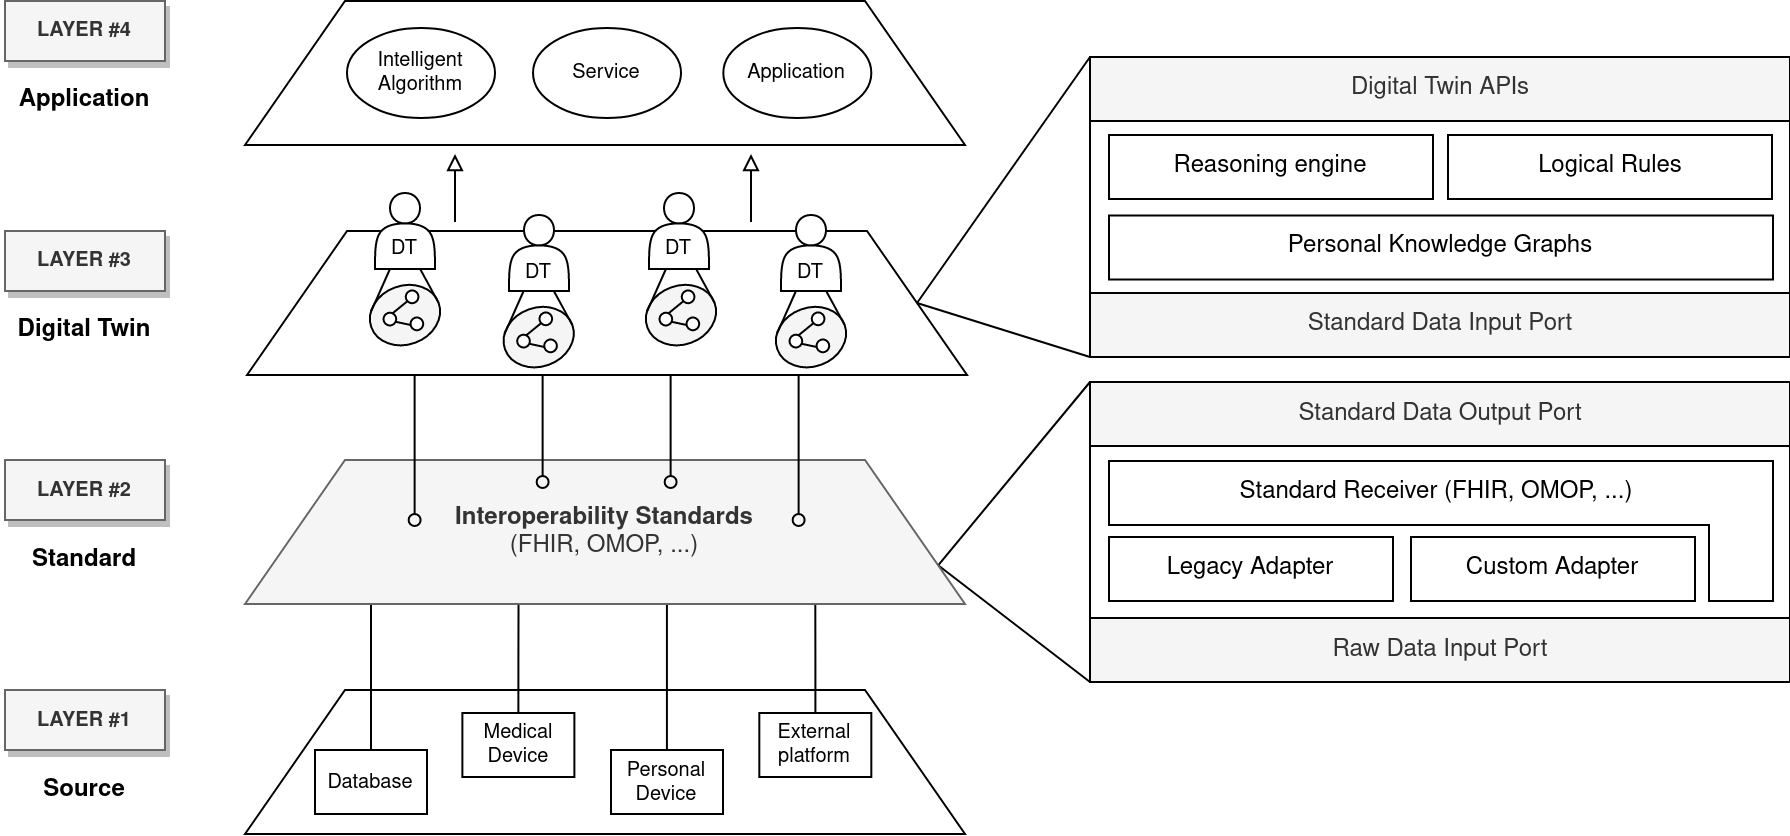
\includegraphics[width=\textwidth]{figures/paper4/Connected.png}
\end{center}
\caption{Illustration depicting the 4-tier architecture's former setup: data from the Physical Assets, modeled using FHIR resources, feed the state of the DTs for the overlying applications and services.}
\label{paper4_fig1}
\end{figure}

CONNECTED is designed in a microservices architectural style which consists of dividing services into a set of small services. Microservices architecture is considered well-suited for the modular development of flexible, evolving, and distributed systems such as the proposed architecture. Indeed, the microservices architecture offers elasticity. This is manifested in the ability to update the DT framework frequently during runtime. This practice reduces the software delivery time and provides the necessary flexibility to respond quickly and effectively to workload changes that edge and cloud resources may experience. Moreover, it enables seamless orchestration among multiple edge and cloud resources.

Considering the wide range of applications, the flexibility in interaction modes, and the evolution of the system, we consider the development of CONNECTED's microservices using the clean architecture pattern \cite{martin2017clean} that allows the separation of business logic from implementation specifications. In this case, the functionalities of the DT are made available externally through the use of adapters that can make use of specific libraries. Any modifications to the adapters will not affect the core logic of the DT.

The correct communication between the various services is an essential element for the functioning of the whole system. Among the most popular solutions for event-driven information exchange, the use of a message queue is particularly effective. In this asynchronous interaction approach, microservices do not dialogue directly with each other as they produce and consume messages by exploiting a central communication bus, favoring scalability, resilience in the event of disruptions of one or more system components, the decoupling of microservices and the flexibility in introducing new microservices into the system without having to make changes to other components. We adopted Apache Kafka, a distributed event streaming platform, the de facto standard for the implementation of message queues in the context of microservices architectures.

In the following section, we propose an enhancement of the existing CONNECTED architecture, integrating ML models with a formal, machine-readable description of their characteristics. This serves as a standard documentation of the models, possibly empowering the framework with additional capabilities, such as seamless integration of new models, and their coordination with existing algorithms or data sources.

\subsection{Representation of Machine Learning models within CONNECTED}\label{sec:paper4_representation}

Representing the DT as a mere repository of real-time data, while sufficient for certain use cases, does not fully utilize the capabilities of this paradigm. To achieve that, it is necessary to enhance our DT by enabling simulations. Therefore, we are actively striving to integrate ML models into our framework.

A recent survey has shown that up to 87\% of well-performing ML projects never get deployed due to integration issues\cite{venturebeat_why_2019}. A solution to this problem is the adoption of an MLOps workflow that promotes a smoother development experience throughout the whole ML lifecycle time. It results in the deployment of plenty of models through web services. These models can be described utilizing reports, i.e. documents that inform researchers, software developers, stakeholders, and interested persons (such as patients) about the specific model adopted, the inputs, the output, what the ML approach performs, and potential technical or ethical problems. A similar approach, using model cards, is suggested by NIH through their Bridge2AI programme to provide informative and transparent descriptions of ML models to stakeholders \cite{Amith2022}. Nonetheless, as a static document, they do limit opportunities to permit the information contained within the report to be computable.
We propose to pair every model with a Manifest: a machine-readable formal description that enriches the model with a detailed explanation of its interface, adopting existing standards and ontologies, such as LOINC, SNOMED-CT, and UOM. It essentially allows us to produce a computable version of the model that can be shared, reused, and linked. The adoption of the Manifest allows for the development of algorithms to automatically index models, aggregate their capabilities, and exploit them to deal with complex tasks. By using an ontology to construct our formal representation of ML models, we standardize the nomenclature and representation of ML model reports, essentially producing a computable version of the model that can be shared, reused, and linked. Manifests are computable artifacts, able to link information about ML models, leverage semantic reasoning to link the information, and open up software tooling opportunities, aggregation of models, and querying of the information for healthcare ML research.

After defining a bespoke ontology aimed at defining model manifests, we enhance CONNECTED by introducing a bridge linking the DT level (Layer 3) with the ML models. Its purpose is to empower the architecture with the ability to execute models. To do so, it parses Manifests and looks for the required ontological concepts within the patient KG, which will be automatically supplied as input to the respective model. 

Consider the integration of a hypothetical clinical ML model within our evolved framework, aimed at predicting an individual's risk of developing cardiovascular disease over the following decade. This model draws insights from a range of health indicators including blood pressure, cholesterol levels, and BMI. Stakeholders operating at Layer 4 can harness the diverse capabilities of this model, tailoring them to align with the distinctive profiles of patients through the use of the DT API. Specifically, the expanded Layer 3 accesses the model Manifest (Figure~\ref{paper4_fig2}), providing comprehensive descriptions of each health parameter using LOINC codes from the CONNECTED ontology. These codes facilitate the retrieval of precise values from the patient KG, essential as inputs for the model's computations (Figure~\ref{paper4_fig3}). Once the model completes its execution, the outcomes are conveyed back to the user in a standardized format via the DT API.

\begin{figure}
\begin{center}
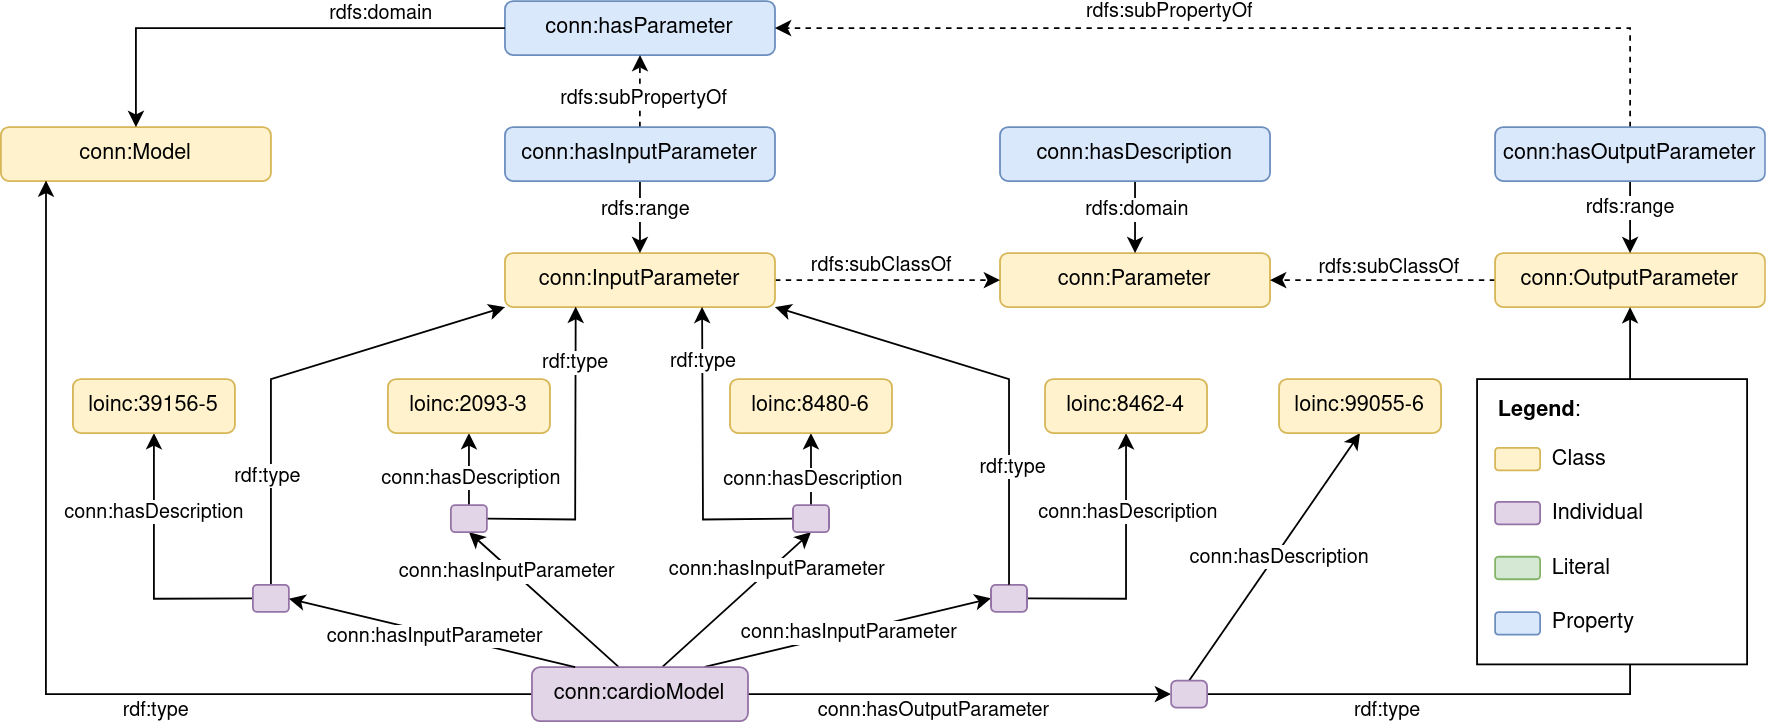
\includegraphics[width=\textwidth]{figures/paper4/connected-ontology-and-model.png}
\end{center}
\caption{RDF Representation of the cardiovascular disease prediction Manifest using the CONNECTED ontology (conn:). It integrates the LOINC ontology terms to uniquely identify the description of the inputs and output of the model.}\label{paper4_fig2}

\end{figure}

\begin{figure}
\begin{center}
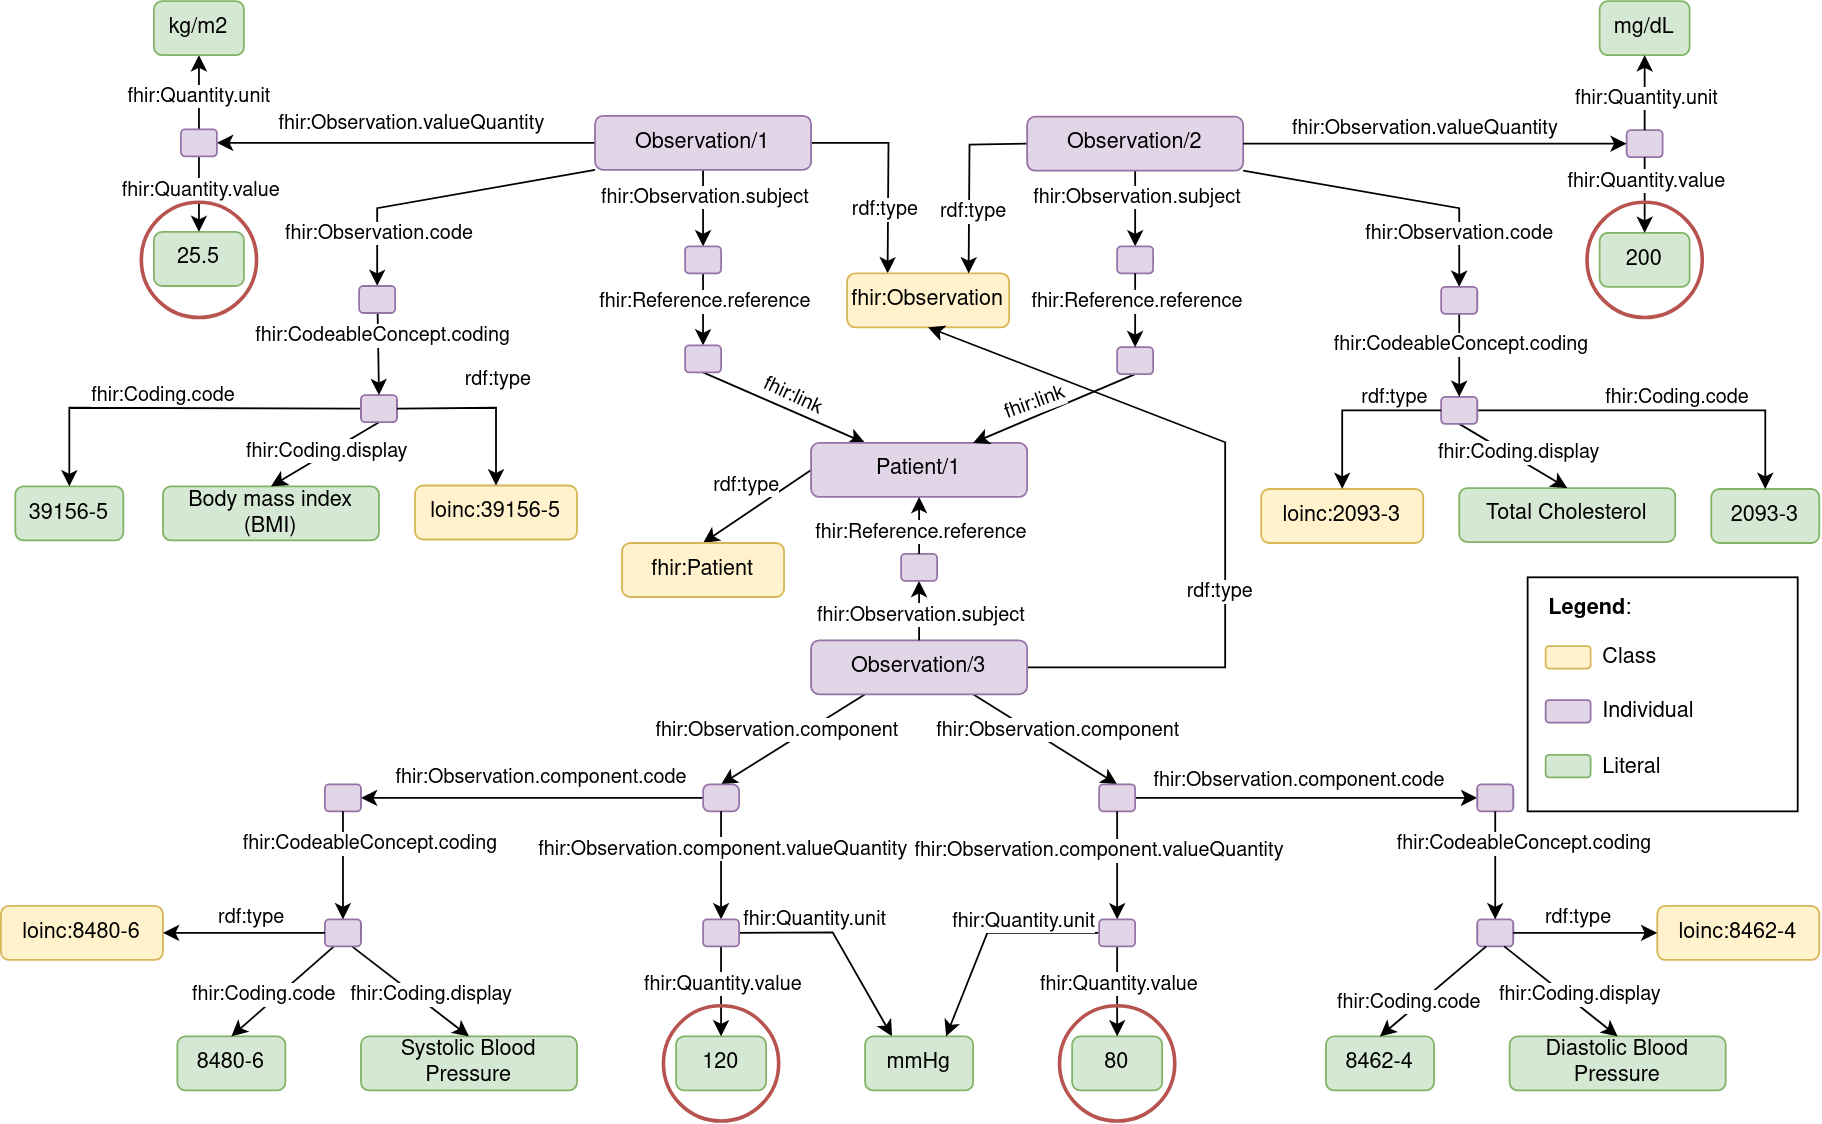
\includegraphics[width=\textwidth]{figures/paper4/patient-fhir-kg.png}
\end{center}
\caption{RDF Representation of a subset of the patient knowledge graph, that uses FHIR/RDF to describe clinical concepts. The marked nodes, being identified by a LOINC code, are those that will be fed to the cardiovascular risk prediction model.}\label{paper4_fig3}
\end{figure}

\subsection{Discussion and Conclusion}\label{sec:paper4_discussion}
This paper proposed the evolution of the CONNECTED conceptual framework, a multi-layered system designed to seamlessly integrate and standardize heterogeneous data sources, facilitating the realization of DTs supported by KGs. Our contribution lies in the introduction of the Manifest concept, which serves as a formal and machine-readable description for ML models, thereby enabling semantic reasoning. This key feature empowers the effective aggregation of these models and facilitates information retrieval regarding their usage. The proposed enhancement not only refines our current vision of DT but also introduces simulation capabilities and an ecosystem where models can be systematically indexed and leveraged. By having a clear description of the models, existing data can be fed automatically to them, improving their overall usability. Some benefits of this approach are: 
\begin{itemize}
    \item Model capabilities described by a document that is independent of a specific language, technology, or framework. 
    \item Detailed and standard description of a model feature, including input/output, through ontologies, dictionaries, etc. 
    \item Automatic/semi-automatic wiring of model input/output with patient data. 
    \item Personalizing generic ML models to specific patient features fosters tailored medicine approach. 
    \item Optionally, create a pipeline of models in which the output of one computation can become the input of the subsequent one. This pipeline could be first validated by matching the types and later executed on specific patients. 
    \item Enabling comparison of different models. 
\end{itemize}
We are applying the proposed extension to some use cases to verify how OWL2-based manifest can represent and formalize ML model information and to show the coverage and usefulness of our proposal in transforming static ML models into a computable format for machine-based processing.

\subsection*{Acknowledgment}
This study was partially supported by the Italian Ministry
of University and Research under PNRR-PNC Project
PNC0000002 ”DARE – Digital Lifelong Prevention” (CUP: B53C22006240001).

% layout: keep this paper's floats within its section
\FloatBarrier
